In this last part, we reflect on the actual competition as well as our own work.
First, \autoref{con:competition} presents the setup and procedure of the competition, as well as the results.
Moreover, some general observations we made while monitoring the behaviour of our agents throughout the matches are given in this section.
\autoref{con:learned} builds upon these observations by explaining in more detail the things we noticed and the conclusions we were able to draw from them.
This section also discusses more general lessons we have learned while developing our multi-agent system.

\subsection{Competition results}
The competition took place on two dates (15th and 17th of September) and each team had to play three times against all other teams. Each simulation consisted of a total of 400 steps and the team with the highest score at the end got three points for a victory. The overall score is the sum over all 400 step scores. The score per step is composed of points for zones plus achievement points. Since the strategy of team "MaKo" was to extensively buy upgrades for the artillery agent", most of the earned achievement points were consumed and therefore did not count towards the step score. Figure \autoref{dis:achievement_points} shows the progress of achievement points over time. As one can see, the achievement points of team "MaKo" go up and down due to the buying actions whereas the the points of the other team increase constantly. 
\begin{figure}[ht]
	\centering
	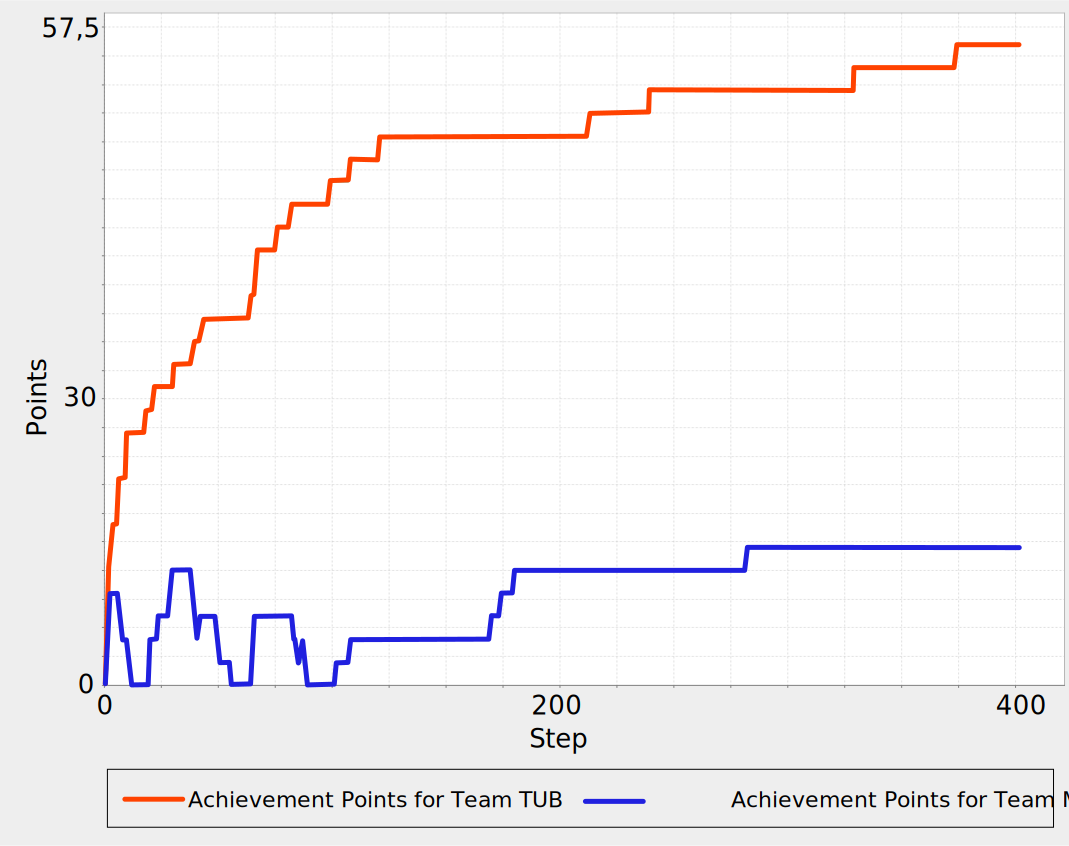
\includegraphics[width=300px]{images/AchievementPoints.png}
	\caption{MAPC 2014 result}
	\label{dis:achievement_points}
\end{figure}
It looks like that this is a huge drawback because achievement points earned at some point count into every future step score. But compared to the number of points awarded for zones, this is only a minor fraction of the step score. As it can be seen in figure \autoref{dis:ZonesScoresAndAchievementPoints} the spending of achievement points paid off since our upgraded saboteur agents hindered the enemy agents from building high valued zones. It was worth spending the achievement points for the purpose of attacking and disturbing the other team because the amount of potential zone points they would have earned without being attacked, is probably much higher than the amount of achievement points team "MaKo" spent for upgrades.
\begin{figure}[h]
	\centering
	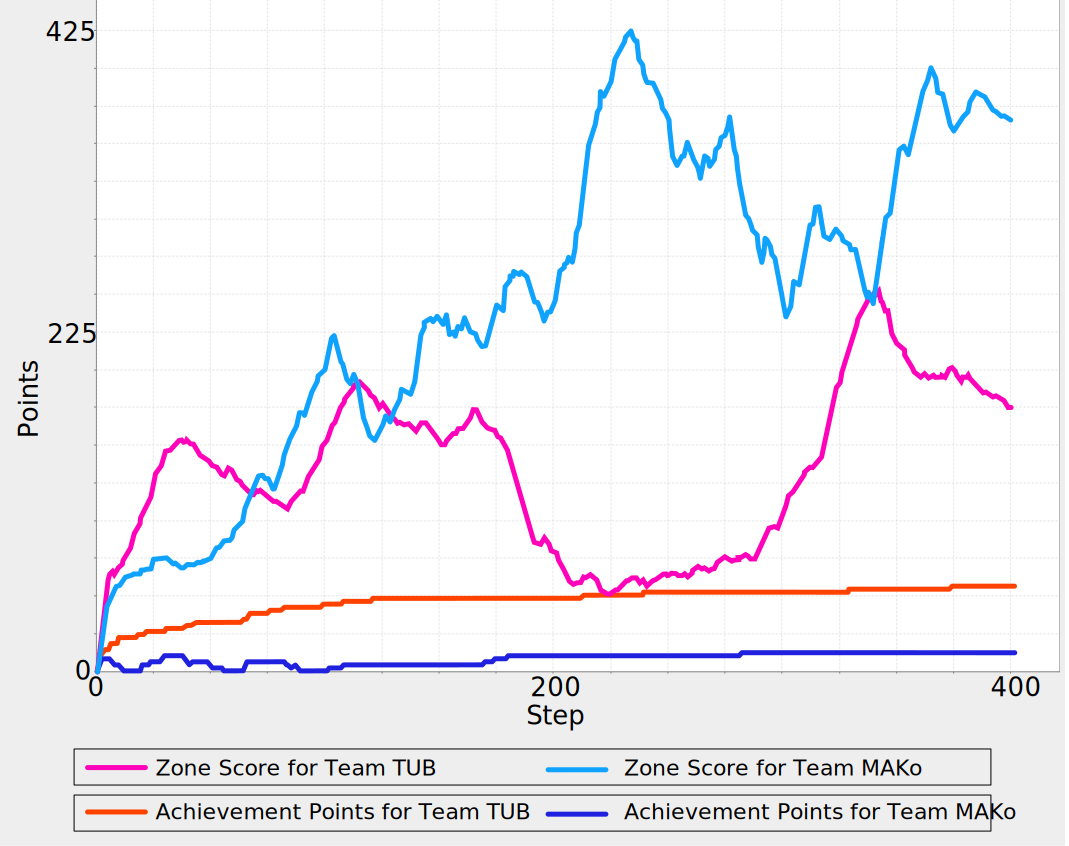
\includegraphics[width=300px]{images/ZonesScoresAndAchievementPoints.png}
	\caption{MAPC 2014 result}
	\label{dis:ZonesScoresAndAchievementPoints}
\end{figure}
At the end of the tournament team "MaKo" scored second with a total of 18 points. The winner 2014 was, for three times in a row now, the team from the USFC. The final results are shown in~\autoref{tab:mapc2014results}.
\begin{table}[ht]
\centering
\caption{The results of the 2014 MAPC. Each team played three matches against every other team, and winning a match awarded 3 points.}
\label{tab:mapc2014results}
\begin{tabular}{@{}lllll@{}}
\toprule
Pos. & Team name      & Score            & Difference            & Points \\ \midrule
1    & SMADAS-UFSC    & 1180662 : 654624 & \phantom{-}526038     & 33     \\
2    & MAKo           & 617086 : 776868  & -15782                & 18     \\
3    & TUB            & 904874 : 872399  & \phantom{-}32475      & 15     \\
4    & TheWonderbolts & 711001 : 1014669 & -303668               & 15     \\
5    & GOAL-DTU       & 653178 : 748241  & -95063                & 9      \\ \bottomrule
\end{tabular}
\end{table}
Statistics of all the individual games can be found in the appendix.[reference here!!!!]

Team "MaKo" lost every second game against each opponent due to the fact that for some reason the repairer agents weren't able to repair. The reason behind this was not obvious to the team. Summarizing the matches, team "MaKo" was capable of exploring the map, building local optima zones, dealing with disabled agents and attacking the opponent. A thing that could be improved is the zoning behaviour. Due to the fact that zones were broken up on a regular basis, zones with a high value sometimes were discarded even when there was no need to do that. Also no handling of edge cases has been implemented which could improve zoning in the sense that the actual number of agents needed to build that zone could be less than the number calculated by our algorithm. But the general idea regarding small zone forming was good. Because one big zone is easy to disturb, having some small high value zones was quite effective to not provide the enemy with an easy target. Like already mentioned a strategy that worked out well, was the approach to upgrade the visibility range and the strength of one saboteur agent significantly. In all matches the it was able to disable enemy agents many times and therefore disturb zones and keep the enemy repairers busy, which kept them away from building zones. 

% TODO: these are from the TOC:
%What place did we rank? How did the others do? Analyse our matches shortly and point out problems we faced, how we tackled them and point out what had gone well.


\subsection{Lessons learned$^{\odot}$}
None of the "MaKo" team member had experience with Jason as a programming language before the research lab.
The first thing that caused problems was that Jason was quite slow, especially when it comes to communication between agents.
Since agents most times needed some information from others and could not continue with their reasoning until this information was given, communication was a extreme bottleneck.
Extreme delay was observed when the group tried to exchange information about the graph.
The first approach was to communicate everything that an agent perceives, while exploring the graph, to every other agent.
The reason behind this was to have every agent store the full knowledge about the until then explored (sub-)graph.
This course of action was quickly discarded, because agents were not able to do actions while processing all the incoming messages.
The next attempt to reduce communication was to implement a so called "cartographer" agent.
The purpose of this agent was to have an additionally agent in the background that gathers all the information about the map that all 28 agents perceive.
With that cartographer agent the amount of communication was reduced and agents could act like intended, because now they just sent their percepts to the cartographer agent and they had not to deal with incoming messages of the other 27 agents.
The drawback of this approach revealed when it came to querying the cartographer agent for information, for instance when an agent wanted to know if a vertex was already surveyed or how he could reach given vertex.
Like it was noticed before, processing the received messages is quite slow and so it happened that the cartographer agent was not able to handle messages in time.
It occurred that agents asked about some specific vertex which the cartographer agent should have known about (because some other agent already informed him about that particular vertex) and they got no answer due to the fact that the cartographer agent hadn't processed the message yet.
That's why this approach was also discarded.
The next idea, which worked in the end, was to use a Java object, the so called "map agent", for the purpose of storing and processing graph information.
Internal actions were used to obtain the required information about the graph.
For instance the internal action "getBestHopToVertex" calculates the shortest path and returns, for a given target node, the next vertex where the agent has to go to.
Another issue that arose initially during the contest was that if a Term in Jason contains a dash, it is interpreted as a Number.
We observed this during our first match against a team that had a dash in its name.
The result was that we were not able to distinguish between friendly and enemy agents.
We immediately fixed it, so that in the next matches we took this possibility of having a dash in the team name into account.

% TODO: these are from the TOC
%Here we could explain what was working well and what was troublesome.  Java: fast.  AS(L): slow and hard for us to program.  Communication: extreme bottleneck.  Also we could note that all this would need much more time and preparation (or a team that is more familiar with agent programming).  %We can illustrate this with our approaches of a dedicated cartographer agent and the node agents.  We might also illustrate further failed approaches.

